% Figure 9: (a) two output channels per DSP48E1 (conv1d_stream g_mul_pack, r7b)
%           (b) decision-feedback look-ahead (dfe_stream.sv, r8c: stages I, A, B)
\documentclass[border=1pt]{standalone}
% Shared style for the report's TikZ diagrams (compiled with Tectonic / XeLaTeX).
% Text in Arial (as in the Word report), mathematics in Computer Modern (as in the matplotlib figures).
\usepackage{fontspec}
\setmainfont{Arial}
\setsansfont{Arial}
\usepackage{amsmath}
\usepackage{tikz}
\usetikzlibrary{arrows.meta,positioning,calc,fit,backgrounds,shapes.geometric,decorations.pathreplacing,shadows}
\hyphenpenalty=10000 \exhyphenpenalty=10000
\definecolor{navy}{HTML}{1F3864}
\definecolor{blue}{HTML}{2E75B6}
\definecolor{light}{HTML}{D9E2F3}
\definecolor{pale}{HTML}{EAF1FB}
\definecolor{orange}{HTML}{C55A11}
\definecolor{paleorange}{HTML}{FFF4E8}
\definecolor{brown}{HTML}{7F3A0B}
\definecolor{green}{HTML}{2E8B57}
\definecolor{palegreen}{HTML}{E8F5EE}
\definecolor{darkgreen}{HTML}{1D5C3A}
\definecolor{gray}{HTML}{7F7F7F}
\definecolor{lgray}{HTML}{BFBFBF}
\definecolor{paleg}{HTML}{F2F2F2}
\definecolor{red}{HTML}{C00000}
\definecolor{txt}{HTML}{333333}
\tikzset{
  >={Stealth[length=1.6mm,width=1.2mm]},
  every node/.style={font=\fontsize{7}{8.4}\selectfont, text=txt},
  blk/.style={draw=blue, fill=white, rounded corners=1.2pt, line width=0.6pt, align=center, inner sep=2.2pt},
  hd/.style={font=\fontsize{7.2}{8.6}\selectfont\bfseries, text=navy},
  sub/.style={font=\fontsize{6.2}{7.4}\selectfont, text=txt},
  wire/.style={->, draw=navy, line width=0.6pt},
  bus/.style={->, draw=navy, line width=1.2pt},
  reg/.style={draw=navy, fill=light, line width=0.5pt, minimum width=1.6mm},
  note/.style={font=\fontsize{6.3}{7.6}\selectfont, text=txt, align=left},
  tag/.style={font=\fontsize{7.6}{9}\selectfont\bfseries, text=navy, anchor=west},
}

\begin{document}
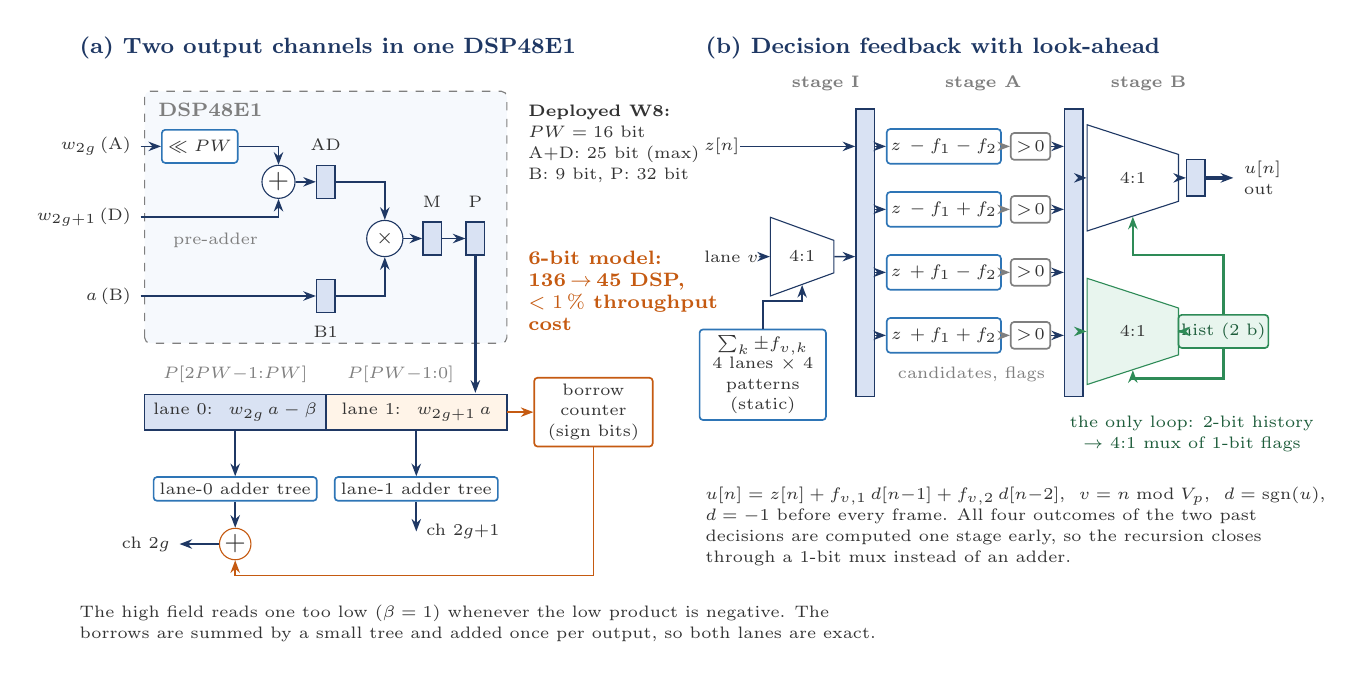
\begin{tikzpicture}[x=1cm,y=1cm]
% ------------------------------------------------------------------ (a) DSP packing
\node[tag] at (-0.1,6.2) {(a) Two output channels in one DSP48E1};
\draw[gray, dashed, rounded corners=2pt, fill=pale!45] (0.85,2.45) rectangle (5.45,5.65);
\node[font=\fontsize{6.6}{8}\selectfont\bfseries, text=gray, anchor=north west] at (0.9,5.62) {DSP48E1};
% ports
\node[anchor=east, sub] (wa) at (0.8,4.95) {$w_{2g}$\,(A)};
\node[anchor=east, sub] (wd) at (0.8,4.05) {$w_{2g+1}$\,(D)};
\node[anchor=east, sub] (ab) at (0.8,3.05) {$a$\,(B)};
\node[blk, minimum width=0.85cm, minimum height=0.42cm, sub] (sh) at (1.55,4.95) {$\ll PW$};
\node[circle, draw=navy, fill=white, inner sep=0.5pt, minimum size=0.42cm, font=\bfseries] (pa) at (2.55,4.5) {$+$};
\node[reg, minimum height=0.42cm] (rad) at (3.15,4.5) {};
\node[reg, minimum height=0.42cm] (rb) at (3.15,3.05) {};
\node[circle, draw=navy, fill=white, inner sep=0.5pt, minimum size=0.46cm] (mu) at (3.9,3.78) {$\times$};
\node[reg, minimum height=0.42cm] (rm) at (4.5,3.78) {};
\node[reg, minimum height=0.42cm] (rp) at (5.05,3.78) {};
\node[sub, above=0.5mm of rad] {AD};
\node[sub, below=0.4mm of rb] {B1};
\node[sub, above=0.5mm of rm] {M};
\node[sub, above=0.5mm of rp] {P};
\node[sub, text=gray, anchor=north] at (1.75,3.98) {pre-adder};
\draw[wire] (wa) -- (sh);
\draw[wire] (sh.east) -| (pa.north);
\draw[wire] (wd) -| (pa.south);
\draw[wire] (pa) -- (rad);
\draw[wire] (ab) -- (rb);
\draw[wire] (rad.east) -| (mu.north);
\draw[wire] (rb.east) -| (mu.south);
\draw[wire] (mu) -- (rm);
\draw[wire] (rm) -- (rp);
% P split into two lanes
\draw[bus] (rp.south) -- (5.05,1.82);
\fill[light] (0.85,1.35) rectangle (3.15,1.8);
\fill[paleorange] (3.15,1.35) rectangle (5.45,1.8);
\draw[navy, line width=0.6pt] (0.85,1.35) rectangle (5.45,1.8);
\draw[navy, line width=0.6pt] (3.15,1.35) -- (3.15,1.8);
\node[sub] at (2.0,1.575) {lane 0: \ $w_{2g}\,a - \beta$};
\node[sub] at (4.3,1.575) {lane 1: \ $w_{2g+1}\,a$};
\node[sub, text=gray, anchor=south] at (2.0,1.82) {$P[2PW{-}1{:}PW]$};
\node[sub, text=gray, anchor=south] at (4.1,1.82) {$P[PW{-}1{:}0]$};
% trees
\node[blk, sub, minimum width=2.0cm] (t0) at (2.0,0.6) {lane-0 adder tree};
\node[blk, sub, minimum width=2.0cm] (t1) at (4.3,0.6) {lane-1 adder tree};
\node[blk, sub, draw=orange, text width=1.35cm] (bc) at (6.55,1.575) {borrow counter\\(sign bits)};
\node[circle, draw=orange, fill=white, inner sep=0.4pt, minimum size=0.36cm, font=\bfseries] (pb) at (2.0,-0.1) {$+$};
\draw[wire] (2.0,1.35) -- (t0);
\draw[wire] (4.3,1.35) -- (t1);
\draw[wire, orange] (5.45,1.575) -- (bc.west);
\draw[wire, orange] (bc.south) |- (2.0,-0.5) -- (pb.south);
\draw[wire] (t0) -- (pb);
\draw[wire] (pb.west) -- ++(-0.5,0) node[left, sub] {ch $2g$};
\draw[wire] (t1.south) -- ++(0,-0.38) node[right, sub, anchor=west] {ch $2g{+}1$};
% notes (right column)
\node[note, anchor=north west] at (5.6,5.6) {\textbf{Deployed W8:}\\$PW = 16$ bit\\A$+$D: 25 bit (max)\\B: 9 bit, P: 32 bit};
\node[note, anchor=north west, text=orange, font=\fontsize{6.6}{8}\selectfont\bfseries] at (5.6,3.75) {6-bit model:\\136\,$\to$\,45 DSP,\\$<1\,\%$ throughput\\cost};
\node[note, anchor=north west] at (-0.1,-0.75) {The high field reads one too low ($\beta = 1$) whenever the low product is negative. The\\borrows are summed by a small tree and added once per output, so both lanes are exact.};

% ------------------------------------------------------------------ (b) DFE look-ahead
\begin{scope}[xshift=7.95cm]
\node[tag] at (-0.1,6.2) {(b) Decision feedback with look-ahead};
\foreach \x/\s in {1.55/stage I, 3.55/stage A, 5.65/stage B}
  \node[font=\fontsize{6.4}{7.6}\selectfont\bfseries, text=gray] at (\x,5.75) {\s};
% inputs
\node[anchor=west, sub, inner xsep=0pt] (z) at (0.0,4.95) {$z[n]$};
\node[anchor=west, sub, inner xsep=0pt] (v) at (0.0,3.55) {lane $v$};
\node[blk, sub, text width=1.45cm] (tab) at (0.75,2.05) {$\sum_k \pm f_{v,k}$\\4 lanes $\times$ 4\\patterns (static)};
\node[trapezium, trapezium angle=70, shape border rotate=270, draw=navy, fill=white, minimum height=0.5cm, minimum width=1.0cm, inner sep=1pt, sub] (lm) at (1.25,3.55) {4:1};
\draw[wire] (v) -- (lm);
\draw[wire] (tab.north) |- ++(0.5,0.35) -| (lm.south);
% register column I
\node[reg, minimum height=3.65cm] (ri) at (2.05,3.6) {};
\draw[wire] (z) -- (z -| ri.west);
\draw[wire] (lm) -- (lm -| ri.west);
% stage A: four candidates
\foreach \k/\p in {0/{-f_1-f_2},1/{-f_1+f_2},2/{+f_1-f_2},3/{+f_1+f_2}} {
  \pgfmathsetmacro{\yy}{4.95-0.8*\k}
  \node[blk, sub, minimum width=1.45cm, minimum height=0.44cm, inner sep=1pt] (c\k) at (3.05,\yy) {$z\,\p$};
  \node[blk, sub, draw=gray, minimum width=0.5cm, minimum height=0.34cm, inner sep=0.8pt] (g\k) at (4.15,\yy) {$>\!0$};
  \draw[wire] (ri.east |- c\k) -- (c\k);
  \draw[wire, gray] (c\k.east) -- (g\k.west);
}
\node[reg, minimum height=3.65cm] (ra) at (4.7,3.6) {};
\foreach \k in {0,1,2,3} \draw[wire] (g\k.east) -- (g\k.east -| ra.west);
\node[sub, text=gray] at (3.4,2.05) {candidates, flags};
% stage B
\node[trapezium, trapezium angle=72, shape border rotate=270, draw=navy, fill=white, minimum height=0.5cm, minimum width=1.35cm, inner sep=1pt, sub] (cm) at (5.45,4.55) {4:1};
\node[trapezium, trapezium angle=72, shape border rotate=270, draw=green, fill=palegreen, minimum height=0.5cm, minimum width=1.35cm, inner sep=1pt, sub] (fm) at (5.45,2.6) {4:1};
\draw[wire] (ra.east |- cm) -- (cm);
\draw[wire, green] (ra.east |- fm) -- (fm);
\node[reg, minimum height=0.46cm] (ru) at (6.25,4.55) {};
\draw[wire] (cm) -- (ru);
\draw[bus] (ru.east) -- ++(0.35,0) node[right, sub, align=left] {$u[n]$\\out};
\node[blk, draw=green, fill=palegreen, sub, minimum width=0.85cm, minimum height=0.42cm, text=darkgreen, inner sep=1pt] (hist) at (6.6,2.6) {hist (2 b)};
\draw[wire, green, line width=0.9pt] (fm) -- (hist);
\draw[wire, green, line width=0.9pt] (hist.south) -- ++(0,-0.38) -| (fm.south);
\draw[wire, green, line width=0.9pt] (hist.north) -- ++(0,0.75) -| (cm.south);
\node[sub, text=darkgreen, align=center] at (6.2,1.3) {the only loop: 2-bit history\\$\to$ 4:1 mux of 1-bit flags};
% equation
\node[note, anchor=north west] at (-0.1,0.75) {$u[n] = z[n] + f_{v,1}\,d[n{-}1] + f_{v,2}\,d[n{-}2]$, \ $v = n \bmod V_p$, \ $d = \mathrm{sgn}(u)$,\\$d = -1$ before every frame. All four outcomes of the two past\\decisions are computed one stage early, so the recursion closes\\through a 1-bit mux instead of an adder.};
\end{scope}
\end{tikzpicture}
\end{document}
